\section{第一周}
\subsection{写在前面}
概率论与数理统计(吉林大学) 主要学习概率论相关知识,针对数理统计相关内容只做少量介绍不作重点考察.
本课程为16周(每周两节课) 有两次月考.
\subsubsection*{前言}
在日常生活中,我们常常会经历各种事件:太阳从东方升起,购买福利彩票是否中奖等等.这些事情都离不开概率论.我们通常称一定发生的事情为必然事件,有可能发生的事件为随机事件,不可能发生的事情为不可能事件.这是在高中期间我们所学的知识.
\subsubsection*{可列集}
若存在一个映射\(\varphi\)从集合A到自然数集的任一子集(包括自然数集自身)是双射,那么称集合A是可列集.
\subsection{随机现象}
在一定条件下,并不是总出现相同结果的现象称为随机现象.随机现象有两个特点
\begin{itemize}
    \item 结果不止一个 \\
    \item 无法预知结果
\end{itemize}
只有一个结果的现象称为确定性现象.下面我们给出随机现象和确定性现象的例子
\begin{Example}\label{例子1}
    (1) 太阳从东方升起 \\
    (2) 吉林大学是专科学校 \\
    (3) 抛一枚硬币 \\
    (4) 某种手机的电池寿命 
\end{Example}
不难看出例\ref{例子1}的(1),(2)是确定性现象,(3),(4)是随机现象 .在日常生活中随机现象随处可见.对于在相同条件下可以重复的随机现象的观察、记录、实验称为随机试验. 
\subsection{样本空间}
根据随机现象的定义,我们可以知道:随机现象的结果不止一个.我们称随机现象的一切可能基本结果组成的集合为样本空间,记作\(\Omega = \left\{\omega\right\}\),其中\(\omega\)表示基本结果,又称为样本点.就想米是长度的基本单位一样,样本点就是今后在概率论(抽样)中最基本的单位.在认识随机现象时,首先就应该明确该随机现象的样本空间.下面给出例子\ref{例子1}的样本空间 
\begin{Example}
    (1) \(\Omega = \left\{ \omega\right\}\) ,\(\omega\)指的是太阳从东方升起 \\
    (2) \(\Omega = \left\{\omega\right\}\), \(\omega\)指的是吉林大学是专科学校 \\
    (3) \(\Omega = \left\{ \omega_1 , \omega_2\right\} \) \(\omega_1 ,\omega_2\)分别指的是硬币正面、硬币背面 \\
    (4) \(\Omega = \left\{ \omega_1 \omega_2 \dots \omega_n \dots  \right\} \) 分别指的是不同的使用时间(例如 1个月,2个月 等等) 
\end{Example}
需要注意的点是
\begin{itemize}
    \item 样本空间的元素可以是数,是描述性语言,也可以是其他 \\
    \item 随机现象的样本点至少有两个,如果将必然性现象纳入考虑,那么只有一个样本点的样本空间对应的必然性现象 \\
\end{itemize}
根据样本点的个数来划分样本空间:若样本点的个数是有限的或者是无限可列的样本空间,我们称其是离散样本空间;若样本点的个数是无限不可列的样本空间,我们称其为连续样本空间.
\subsection{随机事件}
我们称样本空间中的某些样本点组成的集合称为随机事件.常记为A,B,C,.... 注意: 
\begin{itemize}
    \item 任一事件是随机事件的一个子集,常常使用一个长方形的表格代表随机事件,任一事件是在长方形中的圆形区域,称这样的图表为维恩(Venn)图\\
    \item 事件发生当且仅当事件中的样本点被激活 \\
    \item 由样本空间单个样本点组成的随机事件称为基本事件,随机事件的最大子集是必然事件,最小子集是不可能事件
\end{itemize}
\subsection{随机变量}
用来表示随机现象结果的变量称为随机变量,常用X,Y,Z表示.随机变量是人们根据对于不同研究方面人为设置的变量.
\subsection{事件之间的关系}
\subsubsection*{包含关系}
若随机事件A的全部样本点均位于随机事件B之内,则称A被包含于B,记为\(A \subset B \)
\begin{figure}[h]
    \centering
    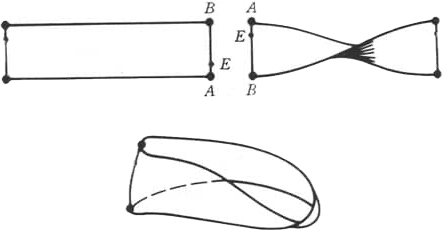
\includegraphics[width=0.5\linewidth]{figures/image_2.png}
    \caption{\(A \subset B \)}
    \label{fig:A belong to B}
\end{figure}
\subsubsection*{相等关系}
若\(A \subset B\)且\(B \subset A\),则称A和B相等,记作\(A = B\)
\subsubsection*{不相容关系}
若不存在样本点既位于A中又位于B中,则称A和B不相容.
\begin{figure}[h]
    \centering
    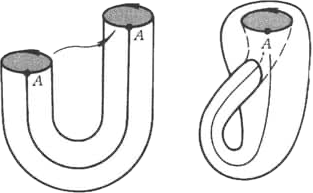
\includegraphics[width=0.5\linewidth]{figures/image_3.png}
    \caption{A和B不相容}
    \label{1}
\end{figure}
\subsection{两个集合的运算}
\subsubsection*{两个集合的交}
由A和B公共的样本点共同组成的随机事件称为A和B的交,用概率论的语言也可以称为A,B共同发生
记为\(A \cap B \)
\begin{Theorem}[乘法原理]
    \(\mathbf{P}(A \cap B)\) = \(\mathbf{P} (A) * \mathbf{P}(B)\)
\end{Theorem}
\subsubsection*{两个集合的并}
由A和B所有的样本点共同组成的随机事件称为A和B的交,用概率论的语言也可以称为A,B至少有一个事件发生 记为\(A \cup B \)
\subsubsection*{两个集合的差}
由A的全体不在B的样本点组成的随机事件称为A和B的差,用概率论的语言也可以称为A发生但是B不发生.记为\(A - B \)
\begin{Definition}[对立事件]
    在样本空间\(\Omega\)中,A的对立事件记为\(\overline{A}\),它的含义是在\(\Omega\)中却不在A中的样本点所组成的随机事件,显而易见的,\[\overline{A} = \Omega - A\]\\
    A与B互为对立事件的充要条件为:\(A\cup B = \Omega\)且\(A \cap B = \varnothing \) 此充要条件也可以称为对立事件的第二定义.
\end{Definition}
要点: 
\begin{itemize}
    \item 对立事件一定是不相容的 , 但是不相容事件不一定是对立事件\\
    \item \(A - B \)可以记为\(A\overline{B}\)
\end{itemize}
\begin{Theorem}[逆向乘法原理]
    \(\mathbf{P}(\overline{A} \cap B)\) = \(1- \mathbf{P}(\overline{A} \cap \overline{B})\)
\end{Theorem}
注意:逆向乘法原理的应用范围比乘法原理要宽广许多,应牢记在心.
\subsection{事件的运算律}
1.结合律
\begin{align}
    (A \cap B) \cap C &= A \cap (B \cap C) \\
    (AB)C &= A(BC)
\end{align}
2.交换律
\begin{align}
    A\cup B &=B \cup A \\
    AB&=BA
\end{align}
3.分配律
\begin{align}
    A\cap (B \cup C) &= AB \cup AC \\
    A\cup(B\cap C ) &= (A \cap B) \cup (A\cap C)
\end{align}
4对偶律(摩根律)
\begin{align}
    \textbf{事件并的对立等于事件对立的交}\overline{(A\cup B)} &= \overline{A} \cap \overline{B} \\
    \textbf{事件交的对立等于事件对立的并 } \overline{(A \cap B )} &= \overline{A} \cup \overline{B}
\end{align}
\subsection{事件域}
此处提出事件域主要是为了接下来定义事件的概率作准备.事件域就是一个样本空间中各种事件加减乘除所构成的空间.因此我们要求这样的事件域一定是运算封闭的.以后记事件域\(\mathcal{F}\) . 通过运算律,我们可以知道: 通过交和对立可以实现差的运算、通过并和对立可以实现交的运算.因此当谈及事件域的运算封闭性时,可以只考虑并和对立.因此得到事件律的定义
\begin{Definition}
    设\(\Omega\)是一个样本空间,\(\mathcal{F}\) 是\(\Omega\)的某些子集构成的集合类,如果\(\mathcal{F}\)满足
    \begin{enumerate}
        \item \(\Omega \in \mathcal{F}\) ; \\
        \item 如果\(A \in \mathcal{F}\),那么\(\overline{A} \in \mathbf{F}\) \\
        \item 如果\(A_k \in \mathcal{F}\),那么它的可列并为\(\bigcup\limits_{k=1}^{\infty} A_K \in \mathcal{F}\)
    \end{enumerate}
则称\(\mathcal{F}\)为\(\Omega\)的一个事件域,又称为\(\sigma\)域或者\(\sigma\)代数
\end{Definition}
但是如果样本空间含有全体实数\(\Omega=(-\infty,+\infty)=\mathcal{R}\),这时事件域\(\mathcal{F}\)中的元素无法一一列出,因此需要通过扩展一个基本集合类来得到上述的样本空间
具体如下:
\begin{itemize}
    \item 取基本集合类\[\mathcal{F} =\left\{(-\infty ,x)| -\infty < x< +\infty \right\}\]\\
    \item 利用事件域对于集合差的运算封闭,得到;\[[a,b) \in \mathcal{F}\] \\
    \item 重复以上操作,我们发现闭区间,单点集,左开又闭区间,开区间都在\(\mathcal{F}\)之内 \\
    \item 通过事件域的运算封闭性,把实数集中的一切有限集,可列集,开集,闭集都扩展进来
\end{itemize}

通过上面操作所得到的全体,我们称为博雷尔事件域,域中的每个元素(集合)都称为博雷尔集,又称为可测集.
\begin{Definition}[样本空间的分割]
    对于样本空间\(\Omega\)来说,如果有n个事件\(D_1,D_2,\dots,D_n\)满足:\[D_i\text{ 互不相交},\bigcup\limits_{i=1}^n D_i = \Omega\] 我们称\(D_i\)是样本空间\(\Omega\)的一组分割\((i=1,2,\dots , n )\),也可以是可列个互不相容的事件\(D_i\)组成\(\Omega\)的一组分割\((i=1,2\dots ,)\)
\end{Definition}
分割主要应用于复杂的概率计算中,通过把一个复杂的样本空间分为数个易于计算的“小”样本空间从而简化运算.